\documentclass[14pt]{extbook}
\usepackage{multicol, enumerate, enumitem, hyperref, color, soul, setspace, parskip, fancyhdr} %General Packages
\usepackage{amssymb, amsthm, amsmath, latexsym, units, mathtools} %Math Packages
\everymath{\displaystyle} %All math in Display Style
% Packages with additional options
\usepackage[headsep=0.5cm,headheight=12pt, left=1 in,right= 1 in,top= 1 in,bottom= 1 in]{geometry}
\usepackage[usenames,dvipsnames]{xcolor}
\usepackage{dashrule}  % Package to use the command below to create lines between items
\newcommand{\litem}[1]{\item#1\hspace*{-1cm}\rule{\textwidth}{0.4pt}}
\pagestyle{fancy}
\lhead{Progress Quiz 5}
\chead{}
\rhead{Version ALL}
\lfoot{8497-6012}
\cfoot{}
\rfoot{Summer C 2021}
\begin{document}

\begin{enumerate}
\litem{
Solve the quadratic equation below. Then, choose the intervals that the solutions belong to, with $x_1 \leq x_2$ (if they exist).\[ -14x^{2} -13 x + 7 = 0 \]\begin{enumerate}[label=\Alph*.]
\item \( x_1 \in [-25.11, -23.76] \text{ and } x_2 \in [22.6, 25.7] \)
\item \( x_1 \in [-0.49, -0.3] \text{ and } x_2 \in [1.1, 3.2] \)
\item \( x_1 \in [-2.86, -1.21] \text{ and } x_2 \in [-0.2, 0.7] \)
\item \( x_1 \in [-6.36, -4.31] \text{ and } x_2 \in [17.4, 19.1] \)
\item \( \text{There are no Real solutions.} \)

\end{enumerate} }
\litem{
Solve the quadratic equation below. Then, choose the intervals that the solutions $x_1$ and $x_2$ belong to, with $x_1 \leq x_2$.\[ 25x^{2} -15 x -54 = 0 \]\begin{enumerate}[label=\Alph*.]
\item \( x_1 \in [-6.12, -5.4] \text{ and } x_2 \in [0.13, 0.59] \)
\item \( x_1 \in [-0.76, -0.47] \text{ and } x_2 \in [3.58, 3.93] \)
\item \( x_1 \in [-4.04, -3.17] \text{ and } x_2 \in [0.47, 0.87] \)
\item \( x_1 \in [-1.58, -0.64] \text{ and } x_2 \in [1.69, 1.98] \)
\item \( x_1 \in [-30.39, -29.06] \text{ and } x_2 \in [44.7, 45.48] \)

\end{enumerate} }
\litem{
Write the equation of the graph presented below in the form $f(x)=ax^2+bx+c$, assuming  $a=1$ or $a=-1$. Then, choose the intervals that $a, b,$ and $c$ belong to.
\begin{center}
    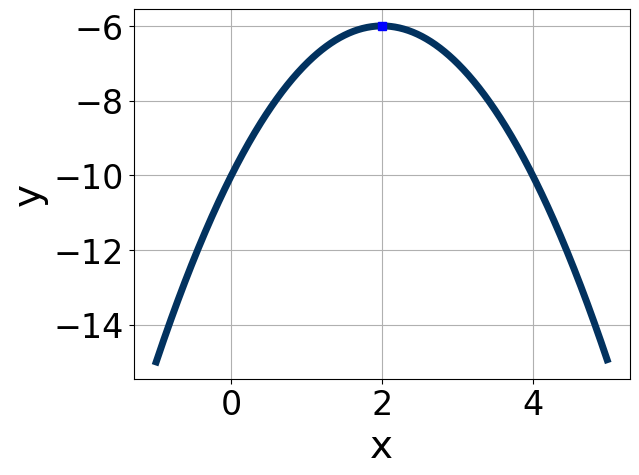
\includegraphics[width=0.5\textwidth]{../Figures/quadraticGraphToEquationCopyA.png}
\end{center}
\begin{enumerate}[label=\Alph*.]
\item \( a \in [-1, 0], \hspace*{5mm} b \in [3, 6], \text{ and } \hspace*{5mm} c \in [-12, -9] \)
\item \( a \in [1, 2], \hspace*{5mm} b \in [-6, -1], \text{ and } \hspace*{5mm} c \in [-2, 0] \)
\item \( a \in [-1, 0], \hspace*{5mm} b \in [-6, -1], \text{ and } \hspace*{5mm} c \in [-12, -9] \)
\item \( a \in [-1, 0], \hspace*{5mm} b \in [-6, -1], \text{ and } \hspace*{5mm} c \in [1, 6] \)
\item \( a \in [1, 2], \hspace*{5mm} b \in [3, 6], \text{ and } \hspace*{5mm} c \in [-2, 0] \)

\end{enumerate} }
\litem{
Factor the quadratic below. Then, choose the intervals that contain the constants in the form $(ax+b)(cx+d); b \leq d.$\[ 24x^{2} +10 x -25 \]\begin{enumerate}[label=\Alph*.]
\item \( a \in [5.71, 7.84], \hspace*{5mm} b \in [-9, -3], \hspace*{5mm} c \in [3.01, 4.8], \text{ and } \hspace*{5mm} d \in [2, 9] \)
\item \( a \in [1.39, 2.74], \hspace*{5mm} b \in [-9, -3], \hspace*{5mm} c \in [11.17, 12.67], \text{ and } \hspace*{5mm} d \in [2, 9] \)
\item \( a \in [-0.34, 1.88], \hspace*{5mm} b \in [-20, -15], \hspace*{5mm} c \in [0.8, 1.94], \text{ and } \hspace*{5mm} d \in [27, 31] \)
\item \( a \in [10.73, 12.47], \hspace*{5mm} b \in [-9, -3], \hspace*{5mm} c \in [1.86, 2.49], \text{ and } \hspace*{5mm} d \in [2, 9] \)
\item \( \text{None of the above.} \)

\end{enumerate} }
\litem{
Solve the quadratic equation below. Then, choose the intervals that the solutions $x_1$ and $x_2$ belong to, with $x_1 \leq x_2$.\[ 10x^{2} -53 x + 36 = 0 \]\begin{enumerate}[label=\Alph*.]
\item \( x_1 \in [0.82, 0.99] \text{ and } x_2 \in [3.18, 4.08] \)
\item \( x_1 \in [0.55, 0.84] \text{ and } x_2 \in [4.16, 4.94] \)
\item \( x_1 \in [0.35, 0.47] \text{ and } x_2 \in [8.74, 9.12] \)
\item \( x_1 \in [8, 8.12] \text{ and } x_2 \in [44.8, 45.7] \)
\item \( x_1 \in [1.46, 1.63] \text{ and } x_2 \in [1.24, 2.58] \)

\end{enumerate} }
\litem{
Solve the quadratic equation below. Then, choose the intervals that the solutions belong to, with $x_1 \leq x_2$ (if they exist).\[ 20x^{2} -13 x -9 = 0 \]\begin{enumerate}[label=\Alph*.]
\item \( x_1 \in [-29.78, -29.25] \text{ and } x_2 \in [28.5, 30.7] \)
\item \( x_1 \in [-1.64, -0.95] \text{ and } x_2 \in [0.1, 0.9] \)
\item \( x_1 \in [-0.54, -0.12] \text{ and } x_2 \in [0.6, 1.5] \)
\item \( x_1 \in [-8.61, -7.69] \text{ and } x_2 \in [19.8, 22.5] \)
\item \( \text{There are no Real solutions.} \)

\end{enumerate} }
\litem{
Factor the quadratic below. Then, choose the intervals that contain the constants in the form $(ax+b)(cx+d); b \leq d.$\[ 54x^{2} +33 x -10 \]\begin{enumerate}[label=\Alph*.]
\item \( a \in [-0.4, 1.2], \hspace*{5mm} b \in [-14, -11], \hspace*{5mm} c \in [0.3, 1.3], \text{ and } \hspace*{5mm} d \in [41, 54] \)
\item \( a \in [17.6, 19], \hspace*{5mm} b \in [-3, 3], \hspace*{5mm} c \in [1.6, 3.3], \text{ and } \hspace*{5mm} d \in [5, 15] \)
\item \( a \in [8.4, 10.1], \hspace*{5mm} b \in [-3, 3], \hspace*{5mm} c \in [5.5, 7], \text{ and } \hspace*{5mm} d \in [5, 15] \)
\item \( a \in [1.3, 5.3], \hspace*{5mm} b \in [-3, 3], \hspace*{5mm} c \in [16.4, 21.1], \text{ and } \hspace*{5mm} d \in [5, 15] \)
\item \( \text{None of the above.} \)

\end{enumerate} }
\litem{
Graph the equation below.\[ f(x) = -(x-3)^2 - 16 \]\begin{enumerate}[label=\Alph*.]
\begin{multicols}{2}\item 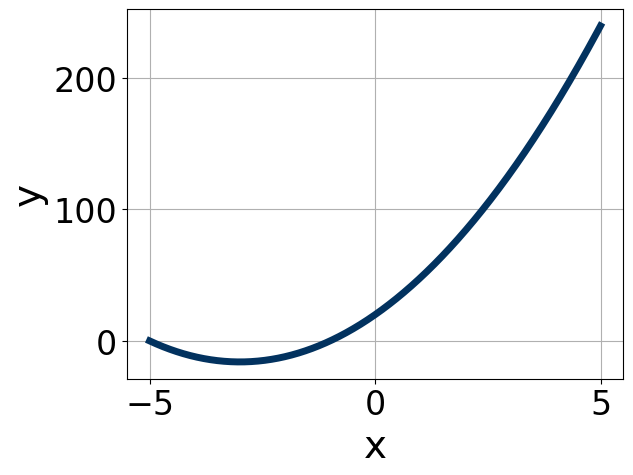
\includegraphics[width = 0.3\textwidth]{../Figures/quadraticEquationToGraphCopyAA.png}\item 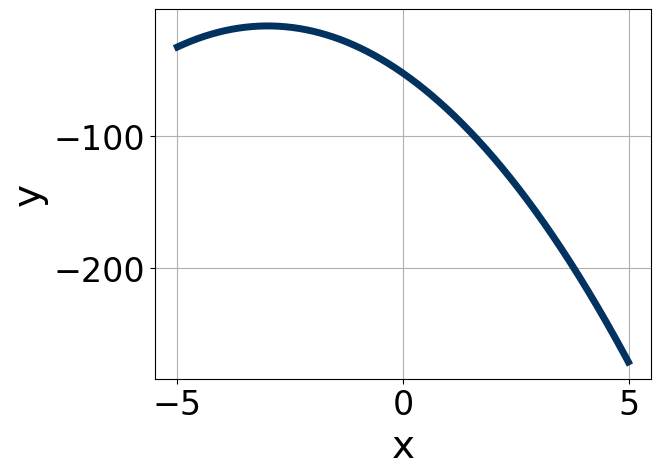
\includegraphics[width = 0.3\textwidth]{../Figures/quadraticEquationToGraphCopyBA.png}\item 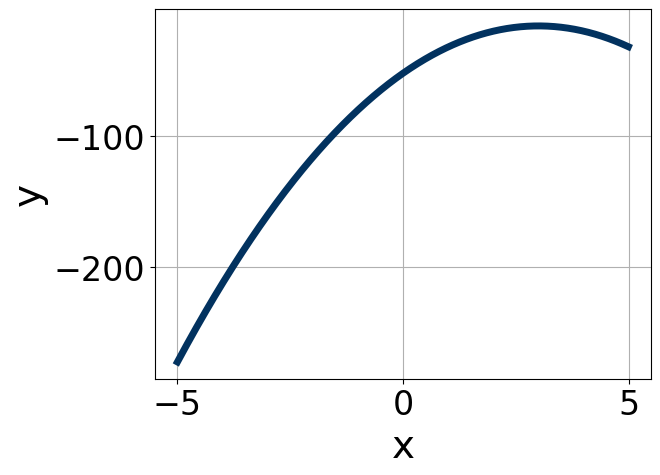
\includegraphics[width = 0.3\textwidth]{../Figures/quadraticEquationToGraphCopyCA.png}\item 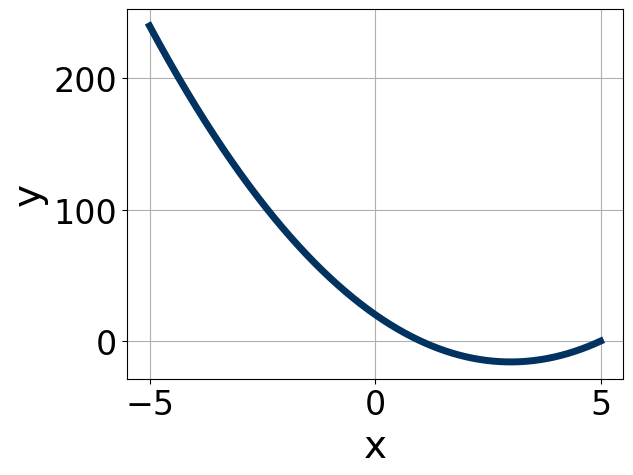
\includegraphics[width = 0.3\textwidth]{../Figures/quadraticEquationToGraphCopyDA.png}\end{multicols}\item None of the above.
\end{enumerate} }
\litem{
Write the equation of the graph presented below in the form $f(x)=ax^2+bx+c$, assuming  $a=1$ or $a=-1$. Then, choose the intervals that $a, b,$ and $c$ belong to.
\begin{center}
    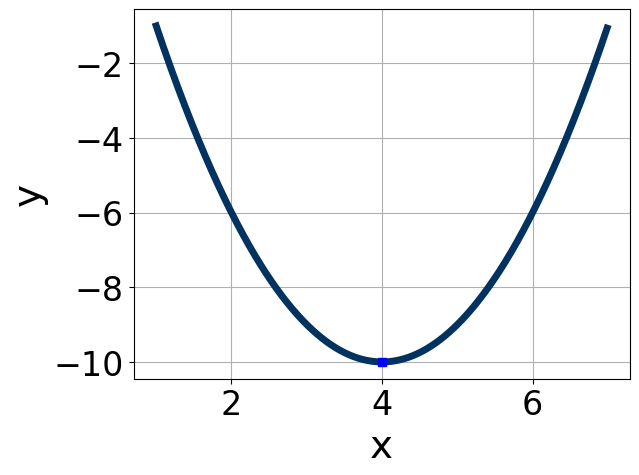
\includegraphics[width=0.5\textwidth]{../Figures/quadraticGraphToEquationA.png}
\end{center}
\begin{enumerate}[label=\Alph*.]
\item \( a \in [0.6, 1.5], \hspace*{5mm} b \in [-11, -6], \text{ and } \hspace*{5mm} c \in [5, 8] \)
\item \( a \in [-1.5, -0.1], \hspace*{5mm} b \in [-11, -6], \text{ and } \hspace*{5mm} c \in [-27, -25] \)
\item \( a \in [0.6, 1.5], \hspace*{5mm} b \in [8, 11], \text{ and } \hspace*{5mm} c \in [5, 8] \)
\item \( a \in [-1.5, -0.1], \hspace*{5mm} b \in [8, 11], \text{ and } \hspace*{5mm} c \in [-27, -25] \)
\item \( a \in [0.6, 1.5], \hspace*{5mm} b \in [8, 11], \text{ and } \hspace*{5mm} c \in [25, 28] \)

\end{enumerate} }
\litem{
Graph the equation below.\[ f(x) = -(x-4)^2 - 13 \]\begin{enumerate}[label=\Alph*.]
\begin{multicols}{2}\item 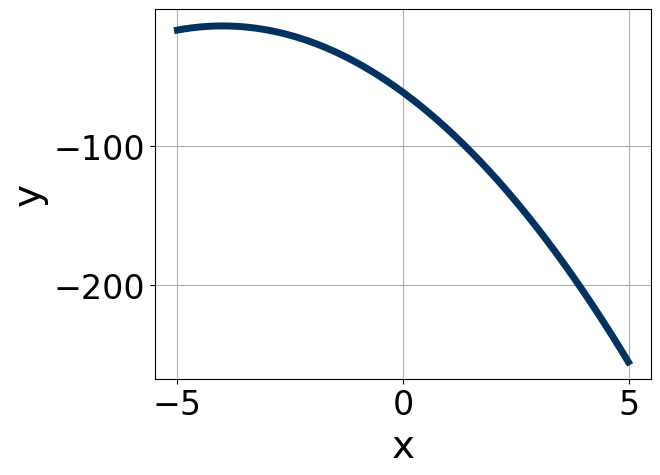
\includegraphics[width = 0.3\textwidth]{../Figures/quadraticEquationToGraphAA.png}\item 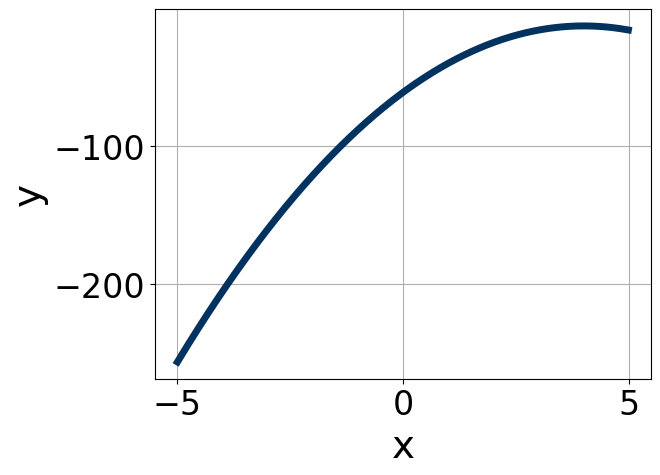
\includegraphics[width = 0.3\textwidth]{../Figures/quadraticEquationToGraphBA.png}\item 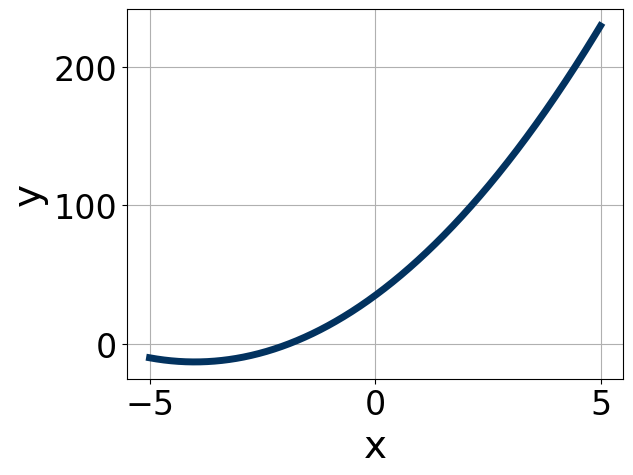
\includegraphics[width = 0.3\textwidth]{../Figures/quadraticEquationToGraphCA.png}\item 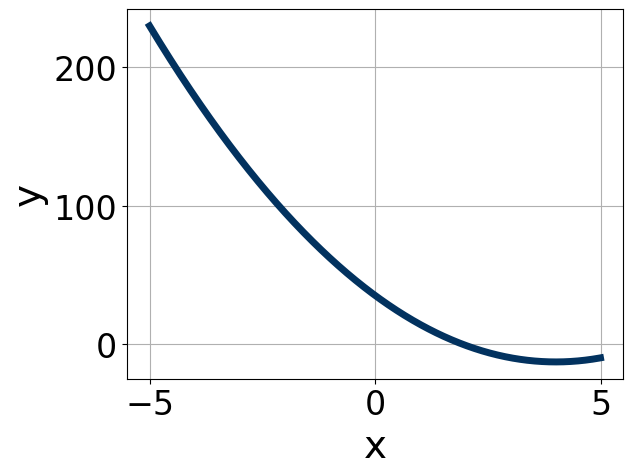
\includegraphics[width = 0.3\textwidth]{../Figures/quadraticEquationToGraphDA.png}\end{multicols}\item None of the above.
\end{enumerate} }
\litem{
Solve the quadratic equation below. Then, choose the intervals that the solutions belong to, with $x_1 \leq x_2$ (if they exist).\[ 17x^{2} +14 x -5 = 0 \]\begin{enumerate}[label=\Alph*.]
\item \( x_1 \in [-0.4, -0.1] \text{ and } x_2 \in [0.71, 1.59] \)
\item \( x_1 \in [-23.6, -21.9] \text{ and } x_2 \in [22.69, 23.43] \)
\item \( x_1 \in [-19.5, -17.5] \text{ and } x_2 \in [3.72, 5.33] \)
\item \( x_1 \in [-2, -0.9] \text{ and } x_2 \in [0.18, 0.3] \)
\item \( \text{There are no Real solutions.} \)

\end{enumerate} }
\litem{
Solve the quadratic equation below. Then, choose the intervals that the solutions $x_1$ and $x_2$ belong to, with $x_1 \leq x_2$.\[ 25x^{2} +60 x + 36 = 0 \]\begin{enumerate}[label=\Alph*.]
\item \( x_1 \in [-30.76, -28.93] \text{ and } x_2 \in [-30, -29.94] \)
\item \( x_1 \in [-1.75, 0.49] \text{ and } x_2 \in [-1.24, -1.14] \)
\item \( x_1 \in [-3.31, -1.72] \text{ and } x_2 \in [-0.87, -0.59] \)
\item \( x_1 \in [-4.53, -2.51] \text{ and } x_2 \in [-0.45, -0.32] \)
\item \( x_1 \in [-7.83, -5.79] \text{ and } x_2 \in [-0.31, -0] \)

\end{enumerate} }
\litem{
Write the equation of the graph presented below in the form $f(x)=ax^2+bx+c$, assuming  $a=1$ or $a=-1$. Then, choose the intervals that $a, b,$ and $c$ belong to.
\begin{center}
    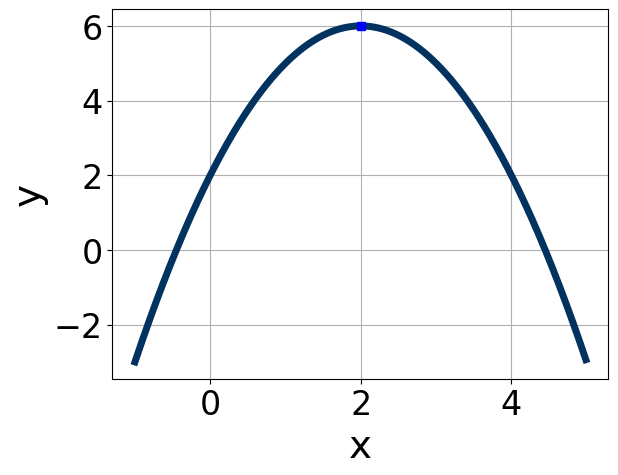
\includegraphics[width=0.5\textwidth]{../Figures/quadraticGraphToEquationCopyB.png}
\end{center}
\begin{enumerate}[label=\Alph*.]
\item \( a \in [-2.8, -0.7], \hspace*{5mm} b \in [-6, -3], \text{ and } \hspace*{5mm} c \in [-11, -9] \)
\item \( a \in [0, 3], \hspace*{5mm} b \in [-6, -3], \text{ and } \hspace*{5mm} c \in [8, 12] \)
\item \( a \in [-2.8, -0.7], \hspace*{5mm} b \in [4, 8], \text{ and } \hspace*{5mm} c \in [1, 3] \)
\item \( a \in [0, 3], \hspace*{5mm} b \in [4, 8], \text{ and } \hspace*{5mm} c \in [8, 12] \)
\item \( a \in [-2.8, -0.7], \hspace*{5mm} b \in [-6, -3], \text{ and } \hspace*{5mm} c \in [1, 3] \)

\end{enumerate} }
\litem{
Factor the quadratic below. Then, choose the intervals that contain the constants in the form $(ax+b)(cx+d); b \leq d.$\[ 36x^{2} +60 x + 25 \]\begin{enumerate}[label=\Alph*.]
\item \( a \in [3.9, 6.6], \hspace*{5mm} b \in [2, 7], \hspace*{5mm} c \in [5.47, 6.34], \text{ and } \hspace*{5mm} d \in [2, 8] \)
\item \( a \in [10.9, 12.9], \hspace*{5mm} b \in [2, 7], \hspace*{5mm} c \in [2.8, 3.1], \text{ and } \hspace*{5mm} d \in [2, 8] \)
\item \( a \in [-0.6, 1.6], \hspace*{5mm} b \in [21, 31], \hspace*{5mm} c \in [0.81, 1.95], \text{ and } \hspace*{5mm} d \in [29, 31] \)
\item \( a \in [1.1, 4.3], \hspace*{5mm} b \in [2, 7], \hspace*{5mm} c \in [9.79, 12.69], \text{ and } \hspace*{5mm} d \in [2, 8] \)
\item \( \text{None of the above.} \)

\end{enumerate} }
\litem{
Solve the quadratic equation below. Then, choose the intervals that the solutions $x_1$ and $x_2$ belong to, with $x_1 \leq x_2$.\[ 10x^{2} -57 x + 54 = 0 \]\begin{enumerate}[label=\Alph*.]
\item \( x_1 \in [0.21, 0.47] \text{ and } x_2 \in [13.33, 14.47] \)
\item \( x_1 \in [1.4, 1.73] \text{ and } x_2 \in [2.3, 3.91] \)
\item \( x_1 \in [0.77, 0.94] \text{ and } x_2 \in [5.55, 7.11] \)
\item \( x_1 \in [1.04, 1.36] \text{ and } x_2 \in [4.17, 5.36] \)
\item \( x_1 \in [11.91, 12.07] \text{ and } x_2 \in [44.83, 45.97] \)

\end{enumerate} }
\litem{
Solve the quadratic equation below. Then, choose the intervals that the solutions belong to, with $x_1 \leq x_2$ (if they exist).\[ 17x^{2} +14 x + 2 = 0 \]\begin{enumerate}[label=\Alph*.]
\item \( x_1 \in [-11.99, -10.69] \text{ and } x_2 \in [-5.1, -3] \)
\item \( x_1 \in [-9.23, -7.19] \text{ and } x_2 \in [7.2, 8.2] \)
\item \( x_1 \in [-0.48, 1.54] \text{ and } x_2 \in [0.3, 1.9] \)
\item \( x_1 \in [-0.93, -0.26] \text{ and } x_2 \in [-0.4, 0.5] \)
\item \( \text{There are no Real solutions.} \)

\end{enumerate} }
\litem{
Factor the quadratic below. Then, choose the intervals that contain the constants in the form $(ax+b)(cx+d); b \leq d.$\[ 24x^{2} -2 x -15 \]\begin{enumerate}[label=\Alph*.]
\item \( a \in [0.3, 2.3], \hspace*{5mm} b \in [-24, -16], \hspace*{5mm} c \in [-0.6, 3.4], \text{ and } \hspace*{5mm} d \in [16, 19] \)
\item \( a \in [2, 3.2], \hspace*{5mm} b \in [-7, -4], \hspace*{5mm} c \in [7.4, 8.3], \text{ and } \hspace*{5mm} d \in [-6, 5] \)
\item \( a \in [17, 21.2], \hspace*{5mm} b \in [-7, -4], \hspace*{5mm} c \in [-0.6, 3.4], \text{ and } \hspace*{5mm} d \in [-6, 5] \)
\item \( a \in [4, 7.3], \hspace*{5mm} b \in [-7, -4], \hspace*{5mm} c \in [3.9, 6.8], \text{ and } \hspace*{5mm} d \in [-6, 5] \)
\item \( \text{None of the above.} \)

\end{enumerate} }
\litem{
Graph the equation below.\[ f(x) = (x+4)^2 + 13 \]\begin{enumerate}[label=\Alph*.]
\begin{multicols}{2}\item 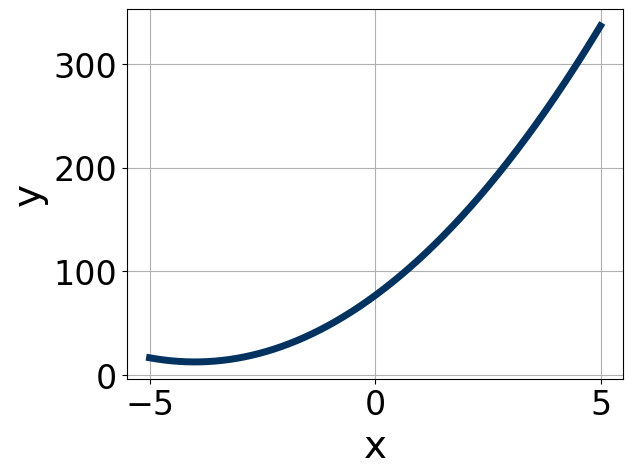
\includegraphics[width = 0.3\textwidth]{../Figures/quadraticEquationToGraphCopyAB.png}\item 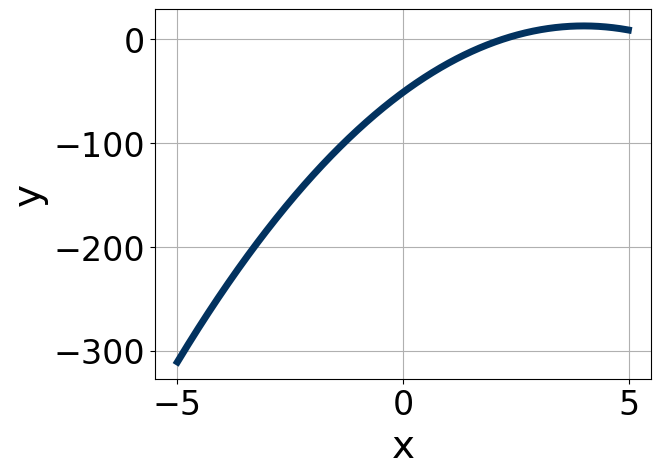
\includegraphics[width = 0.3\textwidth]{../Figures/quadraticEquationToGraphCopyBB.png}\item 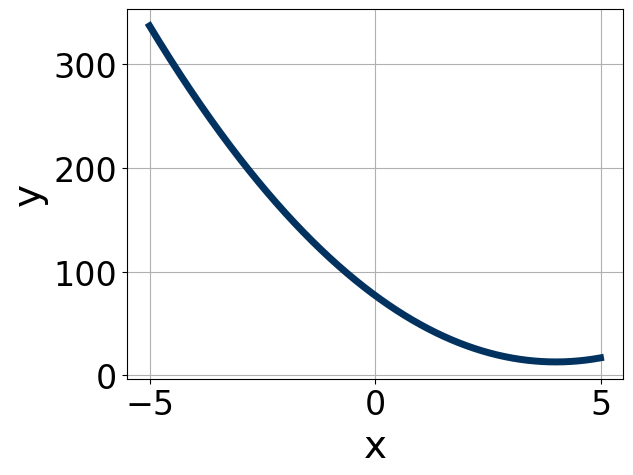
\includegraphics[width = 0.3\textwidth]{../Figures/quadraticEquationToGraphCopyCB.png}\item 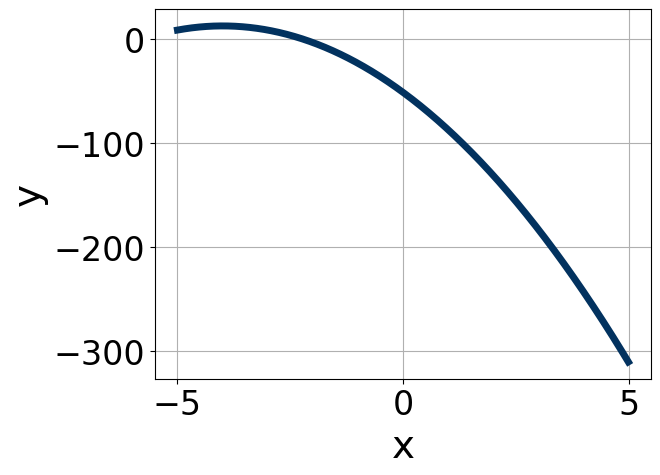
\includegraphics[width = 0.3\textwidth]{../Figures/quadraticEquationToGraphCopyDB.png}\end{multicols}\item None of the above.
\end{enumerate} }
\litem{
Write the equation of the graph presented below in the form $f(x)=ax^2+bx+c$, assuming  $a=1$ or $a=-1$. Then, choose the intervals that $a, b,$ and $c$ belong to.
\begin{center}
    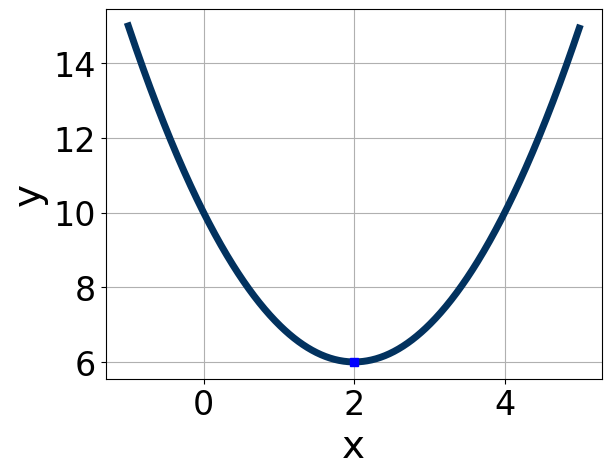
\includegraphics[width=0.5\textwidth]{../Figures/quadraticGraphToEquationB.png}
\end{center}
\begin{enumerate}[label=\Alph*.]
\item \( a \in [0.9, 1.7], \hspace*{5mm} b \in [3, 7], \text{ and } \hspace*{5mm} c \in [8, 11] \)
\item \( a \in [0.9, 1.7], \hspace*{5mm} b \in [3, 7], \text{ and } \hspace*{5mm} c \in [-2, -1] \)
\item \( a \in [-1.2, -0.7], \hspace*{5mm} b \in [3, 7], \text{ and } \hspace*{5mm} c \in [2, 4] \)
\item \( a \in [-1.2, -0.7], \hspace*{5mm} b \in [-4, 0], \text{ and } \hspace*{5mm} c \in [2, 4] \)
\item \( a \in [0.9, 1.7], \hspace*{5mm} b \in [-4, 0], \text{ and } \hspace*{5mm} c \in [8, 11] \)

\end{enumerate} }
\litem{
Graph the equation below.\[ f(x) = -(x-4)^2 - 17 \]\begin{enumerate}[label=\Alph*.]
\begin{multicols}{2}\item 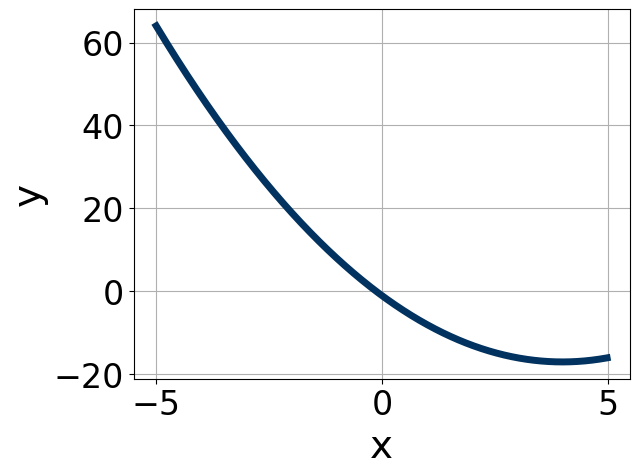
\includegraphics[width = 0.3\textwidth]{../Figures/quadraticEquationToGraphAB.png}\item 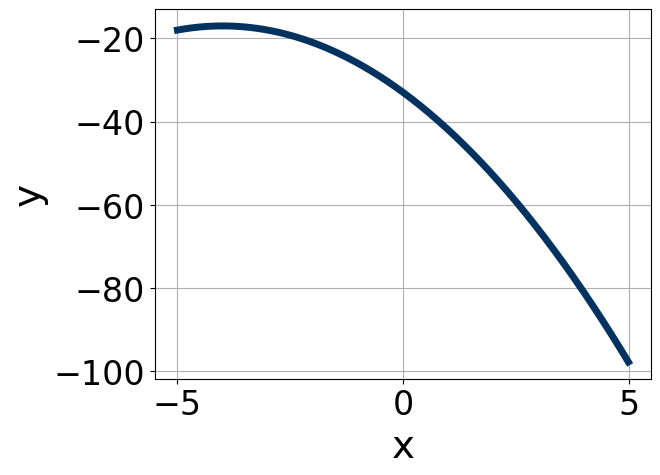
\includegraphics[width = 0.3\textwidth]{../Figures/quadraticEquationToGraphBB.png}\item 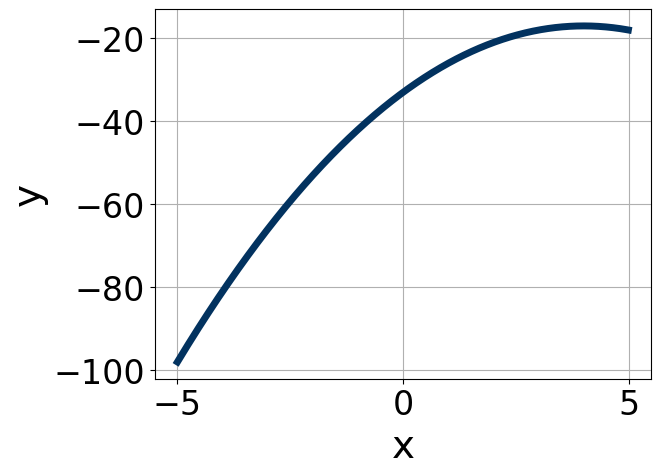
\includegraphics[width = 0.3\textwidth]{../Figures/quadraticEquationToGraphCB.png}\item 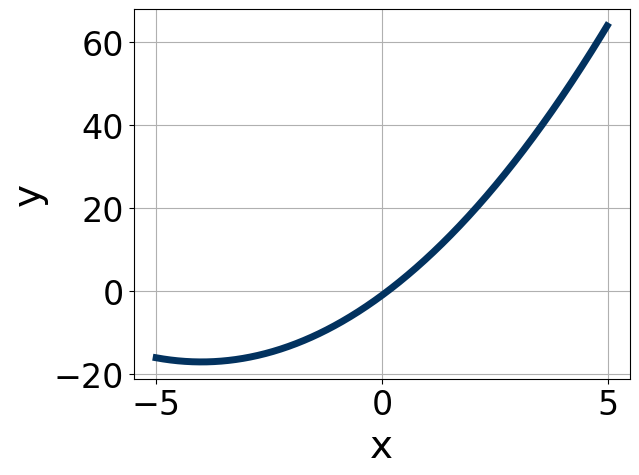
\includegraphics[width = 0.3\textwidth]{../Figures/quadraticEquationToGraphDB.png}\end{multicols}\item None of the above.
\end{enumerate} }
\litem{
Solve the quadratic equation below. Then, choose the intervals that the solutions belong to, with $x_1 \leq x_2$ (if they exist).\[ 11x^{2} +11 x -7 = 0 \]\begin{enumerate}[label=\Alph*.]
\item \( x_1 \in [-16.2, -14.2] \text{ and } x_2 \in [3.1, 6.4] \)
\item \( x_1 \in [-2.4, -1.3] \text{ and } x_2 \in [-0.1, 1] \)
\item \( x_1 \in [-22.2, -21.1] \text{ and } x_2 \in [19.1, 21.3] \)
\item \( x_1 \in [-0.5, 0.9] \text{ and } x_2 \in [0.8, 3.3] \)
\item \( \text{There are no Real solutions.} \)

\end{enumerate} }
\litem{
Solve the quadratic equation below. Then, choose the intervals that the solutions $x_1$ and $x_2$ belong to, with $x_1 \leq x_2$.\[ 25x^{2} -15 x -54 = 0 \]\begin{enumerate}[label=\Alph*.]
\item \( x_1 \in [-6.24, -5.32] \text{ and } x_2 \in [0.19, 0.46] \)
\item \( x_1 \in [-3.77, -3.22] \text{ and } x_2 \in [0.53, 0.91] \)
\item \( x_1 \in [-1.14, -0.1] \text{ and } x_2 \in [5.22, 5.52] \)
\item \( x_1 \in [-2, -1.02] \text{ and } x_2 \in [1.49, 1.96] \)
\item \( x_1 \in [-30.79, -29.91] \text{ and } x_2 \in [44.88, 45.37] \)

\end{enumerate} }
\litem{
Write the equation of the graph presented below in the form $f(x)=ax^2+bx+c$, assuming  $a=1$ or $a=-1$. Then, choose the intervals that $a, b,$ and $c$ belong to.
\begin{center}
    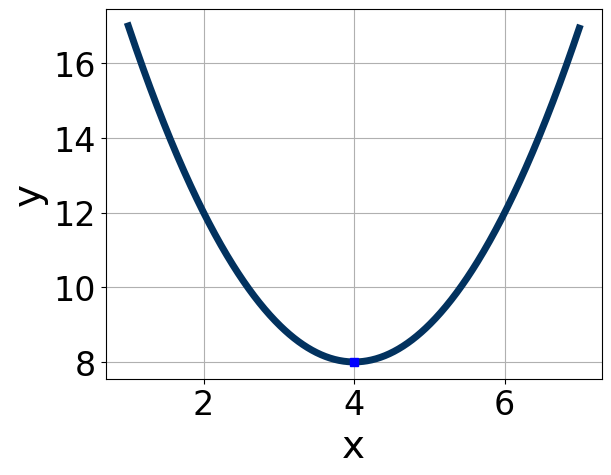
\includegraphics[width=0.5\textwidth]{../Figures/quadraticGraphToEquationCopyC.png}
\end{center}
\begin{enumerate}[label=\Alph*.]
\item \( a \in [0.4, 1.7], \hspace*{5mm} b \in [8, 10], \text{ and } \hspace*{5mm} c \in [7, 10] \)
\item \( a \in [0.4, 1.7], \hspace*{5mm} b \in [-12, -6], \text{ and } \hspace*{5mm} c \in [23, 25] \)
\item \( a \in [0.4, 1.7], \hspace*{5mm} b \in [8, 10], \text{ and } \hspace*{5mm} c \in [23, 25] \)
\item \( a \in [-2.1, -0.5], \hspace*{5mm} b \in [-12, -6], \text{ and } \hspace*{5mm} c \in [-10, -5] \)
\item \( a \in [-2.1, -0.5], \hspace*{5mm} b \in [8, 10], \text{ and } \hspace*{5mm} c \in [-10, -5] \)

\end{enumerate} }
\litem{
Factor the quadratic below. Then, choose the intervals that contain the constants in the form $(ax+b)(cx+d); b \leq d.$\[ 54x^{2} -69 x + 20 \]\begin{enumerate}[label=\Alph*.]
\item \( a \in [17.39, 19.25], \hspace*{5mm} b \in [-7, -4], \hspace*{5mm} c \in [2.94, 4.46], \text{ and } \hspace*{5mm} d \in [-7, 0] \)
\item \( a \in [1.64, 4.34], \hspace*{5mm} b \in [-7, -4], \hspace*{5mm} c \in [26.04, 27.12], \text{ and } \hspace*{5mm} d \in [-7, 0] \)
\item \( a \in [0.38, 1.41], \hspace*{5mm} b \in [-48, -35], \hspace*{5mm} c \in [-0.78, 2.24], \text{ and } \hspace*{5mm} d \in [-27, -22] \)
\item \( a \in [5.38, 6.58], \hspace*{5mm} b \in [-7, -4], \hspace*{5mm} c \in [8.38, 9.36], \text{ and } \hspace*{5mm} d \in [-7, 0] \)
\item \( \text{None of the above.} \)

\end{enumerate} }
\litem{
Solve the quadratic equation below. Then, choose the intervals that the solutions $x_1$ and $x_2$ belong to, with $x_1 \leq x_2$.\[ 15x^{2} +8 x -16 = 0 \]\begin{enumerate}[label=\Alph*.]
\item \( x_1 \in [-3.04, -2.28] \text{ and } x_2 \in [0.32, 0.62] \)
\item \( x_1 \in [-0.72, -0.03] \text{ and } x_2 \in [1.57, 1.93] \)
\item \( x_1 \in [-4.06, -3.53] \text{ and } x_2 \in [0.19, 0.38] \)
\item \( x_1 \in [-20.1, -19.82] \text{ and } x_2 \in [11.94, 12.01] \)
\item \( x_1 \in [-1.53, -0.75] \text{ and } x_2 \in [0.64, 1] \)

\end{enumerate} }
\litem{
Solve the quadratic equation below. Then, choose the intervals that the solutions belong to, with $x_1 \leq x_2$ (if they exist).\[ 17x^{2} -12 x -3 = 0 \]\begin{enumerate}[label=\Alph*.]
\item \( x_1 \in [-3.49, -3.15] \text{ and } x_2 \in [14.83, 15.69] \)
\item \( x_1 \in [-0.77, 0.22] \text{ and } x_2 \in [0.7, 1.97] \)
\item \( x_1 \in [-19.05, -17.7] \text{ and } x_2 \in [17.59, 19.71] \)
\item \( x_1 \in [-1.08, -0.56] \text{ and } x_2 \in [0.04, 0.28] \)
\item \( \text{There are no Real solutions.} \)

\end{enumerate} }
\litem{
Factor the quadratic below. Then, choose the intervals that contain the constants in the form $(ax+b)(cx+d); b \leq d.$\[ 36x^{2} -60 x + 25 \]\begin{enumerate}[label=\Alph*.]
\item \( a \in [5.04, 6.88], \hspace*{5mm} b \in [-6, -3], \hspace*{5mm} c \in [2.7, 6.4], \text{ and } \hspace*{5mm} d \in [-7, -4] \)
\item \( a \in [17.88, 18.99], \hspace*{5mm} b \in [-6, -3], \hspace*{5mm} c \in [1.8, 2.9], \text{ and } \hspace*{5mm} d \in [-7, -4] \)
\item \( a \in [2.15, 3.81], \hspace*{5mm} b \in [-6, -3], \hspace*{5mm} c \in [9, 12.3], \text{ and } \hspace*{5mm} d \in [-7, -4] \)
\item \( a \in [0.87, 1.65], \hspace*{5mm} b \in [-35, -27], \hspace*{5mm} c \in [-1.3, 1.3], \text{ and } \hspace*{5mm} d \in [-33, -21] \)
\item \( \text{None of the above.} \)

\end{enumerate} }
\litem{
Graph the equation below.\[ f(x) = -(x+2)^2 - 16 \]\begin{enumerate}[label=\Alph*.]
\begin{multicols}{2}\item 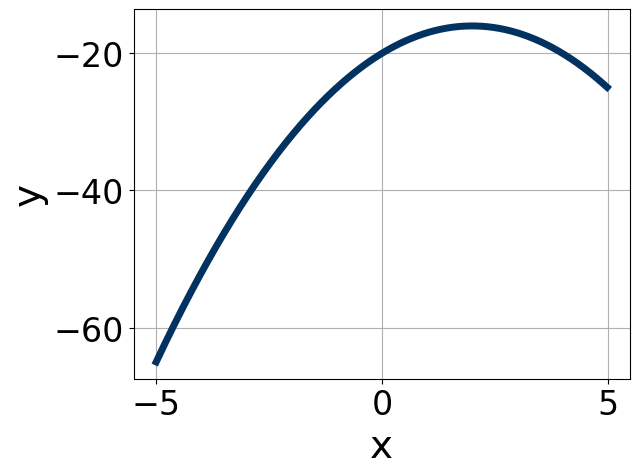
\includegraphics[width = 0.3\textwidth]{../Figures/quadraticEquationToGraphCopyAC.png}\item 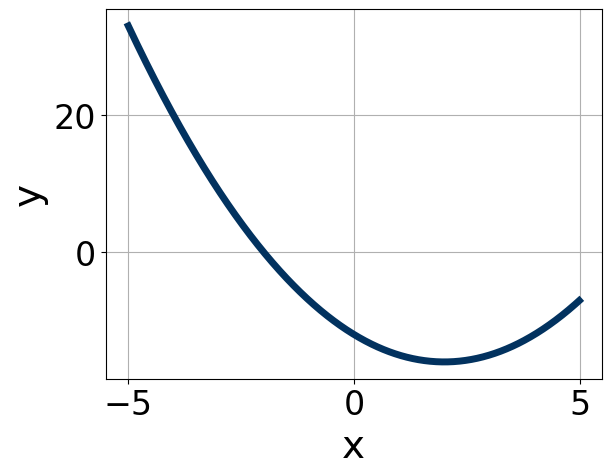
\includegraphics[width = 0.3\textwidth]{../Figures/quadraticEquationToGraphCopyBC.png}\item 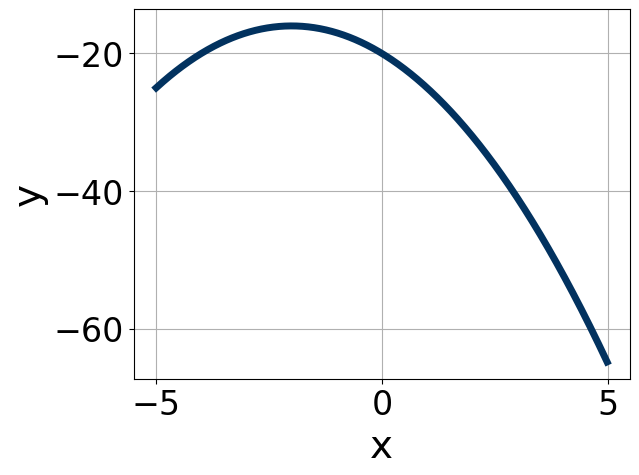
\includegraphics[width = 0.3\textwidth]{../Figures/quadraticEquationToGraphCopyCC.png}\item 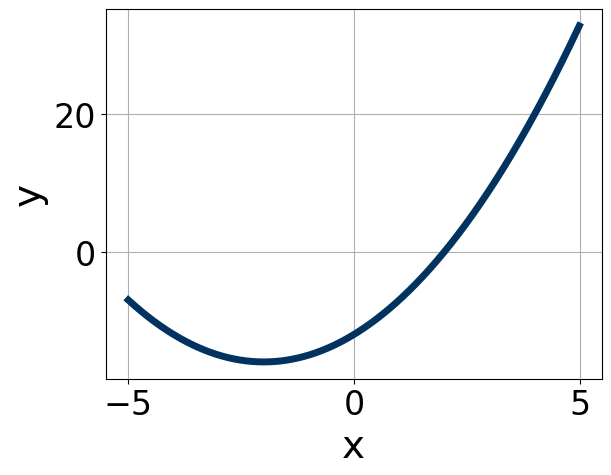
\includegraphics[width = 0.3\textwidth]{../Figures/quadraticEquationToGraphCopyDC.png}\end{multicols}\item None of the above.
\end{enumerate} }
\litem{
Write the equation of the graph presented below in the form $f(x)=ax^2+bx+c$, assuming  $a=1$ or $a=-1$. Then, choose the intervals that $a, b,$ and $c$ belong to.
\begin{center}
    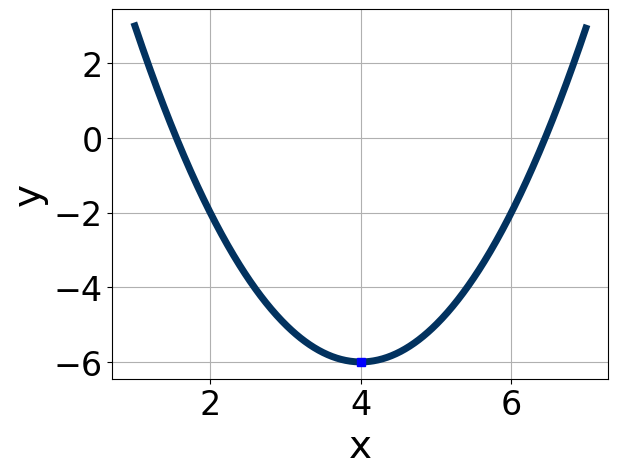
\includegraphics[width=0.5\textwidth]{../Figures/quadraticGraphToEquationC.png}
\end{center}
\begin{enumerate}[label=\Alph*.]
\item \( a \in [0, 4], \hspace*{5mm} b \in [-8, -6], \text{ and } \hspace*{5mm} c \in [7, 14] \)
\item \( a \in [-1, 0], \hspace*{5mm} b \in [-8, -6], \text{ and } \hspace*{5mm} c \in [-24, -21] \)
\item \( a \in [0, 4], \hspace*{5mm} b \in [5, 10], \text{ and } \hspace*{5mm} c \in [7, 14] \)
\item \( a \in [0, 4], \hspace*{5mm} b \in [5, 10], \text{ and } \hspace*{5mm} c \in [21, 23] \)
\item \( a \in [-1, 0], \hspace*{5mm} b \in [5, 10], \text{ and } \hspace*{5mm} c \in [-24, -21] \)

\end{enumerate} }
\litem{
Graph the equation below.\[ f(x) = (x+2)^2 - 17 \]\begin{enumerate}[label=\Alph*.]
\begin{multicols}{2}\item 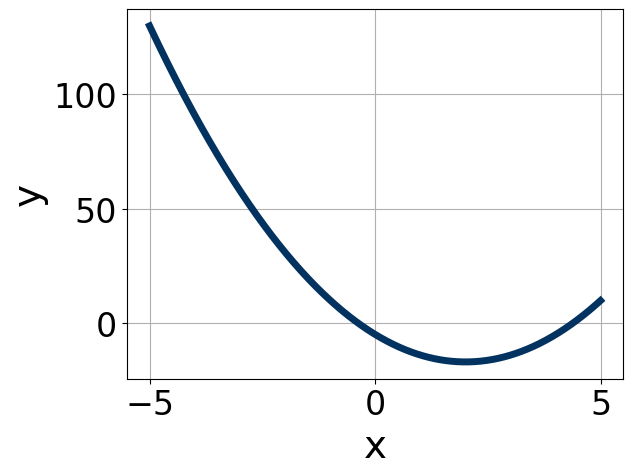
\includegraphics[width = 0.3\textwidth]{../Figures/quadraticEquationToGraphAC.png}\item 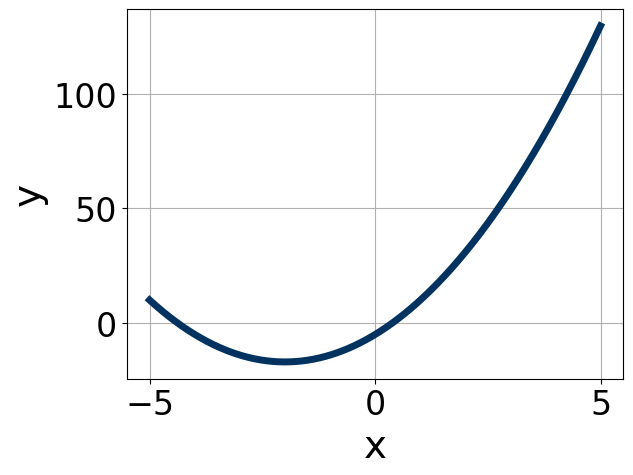
\includegraphics[width = 0.3\textwidth]{../Figures/quadraticEquationToGraphBC.png}\item 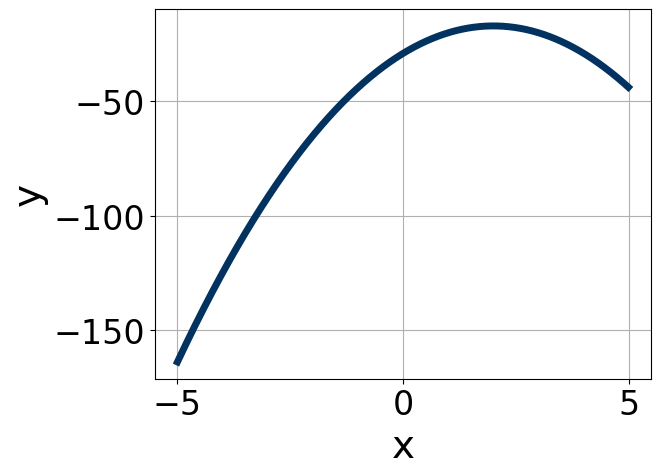
\includegraphics[width = 0.3\textwidth]{../Figures/quadraticEquationToGraphCC.png}\item 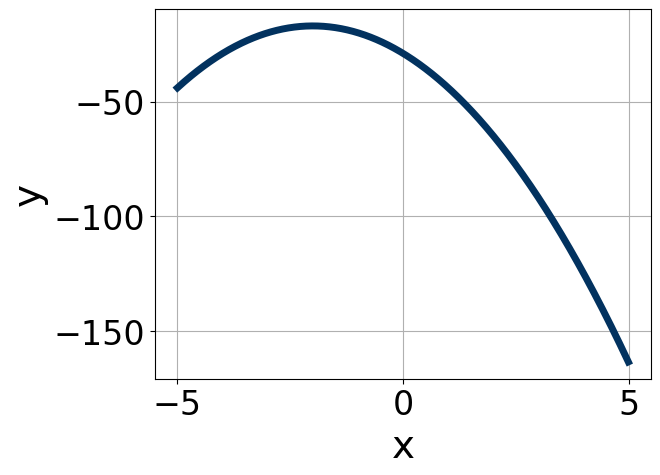
\includegraphics[width = 0.3\textwidth]{../Figures/quadraticEquationToGraphDC.png}\end{multicols}\item None of the above.
\end{enumerate} }
\end{enumerate}

\end{document}